\chapter{REST}

\section{HTTP-verzoekmethoden}

Spring Boot is een goede keuze als je een REST API (of voluit een RESTful web API) wilt ontwikkelen in Java.

REST (Representational State Transfer) is een gestandaardiseerde manier om communicatie tussen verschillende softwaretoepassingen over het internet mogelijk te maken. 
In een RESTful web applicatie wordt de functionaliteit van de applicatie beschikbaar gesteld als resources, die kunnen worden geïdentificeerd door URI's (Uniform Resource Identifiers).  Gebruikers en andere applicaties kunnen met deze resources communiceren via standaard HTTP-verzoekmethoden (HTTP-request, HTTP-method of HTTP-verb). In essentie is HTTP het transportprotocol dat wordt gebruikt om gegevens over te dragen,  terwijl REST de verzameling van ontwerpprincipes is die bepalen hoe die gegevens moeten worden georganiseerd en benaderd.

\begin{itemize}
\item \textbf{GET}: Het GET-verzoek wordt gebruikt om gegevens op te halen van een specifieke resource. 

Voorbeeld URI: GET /api/products/123

Dit verzoek haalt informatie op over het product met ID 123.

\item \textbf{POST}: Het POST-verzoek wordt gebruikt om nieuwe gegevens naar een resource te verzenden. Het wordt vaak gebruikt voor het maken van nieuwe resources of het toevoegen van gegevens aan een bestaande resource.

Voorbeeld URI: POST /api/products

Dit verzoek voegt een nieuw product toe aan de lijst van producten.

\item \textbf{PUT}: Het PUT-verzoek wordt gebruikt om gegevens bij te werken voor een specifieke resource of om een nieuwe resource te maken als deze niet bestaat. Het is idempotent, wat betekent dat meerdere PUT-verzoeken hetzelfde resultaat opleveren.

Voorbeeld URI: PUT /api/products/123

Dit verzoek bijwerken de informatie van het product met ID 123.

\item \textbf{DELETE}: Het DELETE-verzoek wordt gebruikt om een resource te verwijderen of te deactiveren.

Voorbeeld URI: DELETE /api/products/123

Dit verzoek verwijdert het product met ID 123 uit de lijst van producten.
\end{itemize}

\section{Spring Boot Starter Web}

Spring Boot Starter Web is de verzameling van alle bibliotheken (third party libraries) die we nodig hebben om RESTful web applicaties te bouwen.  De verzameling bestaat ondermeer uit Spring MVC,  REST en Tomcat. 
Apache Tomcat is een populaire open source web server voor Java toepassingen.  Als je de dependency spring-boot-start-web toevoegt, start de Tomcat web server op zodra je de Spring boot applicatie opstart.  We spreken van de "embedded web server" in Spring boot.  Je kan er ook voor kiezen om  \'e\'en van de alternatieve web servers te gebruiken zoals jetty of undertow.

\begin{lstlisting}
		<dependency>
			<groupId>org.springframework.boot</groupId>
			<artifactId>spring-boot-starter-web</artifactId>
		</dependency>
		\end{lstlisting}
		
		
By running the main-class you start your Spring Boot application. 

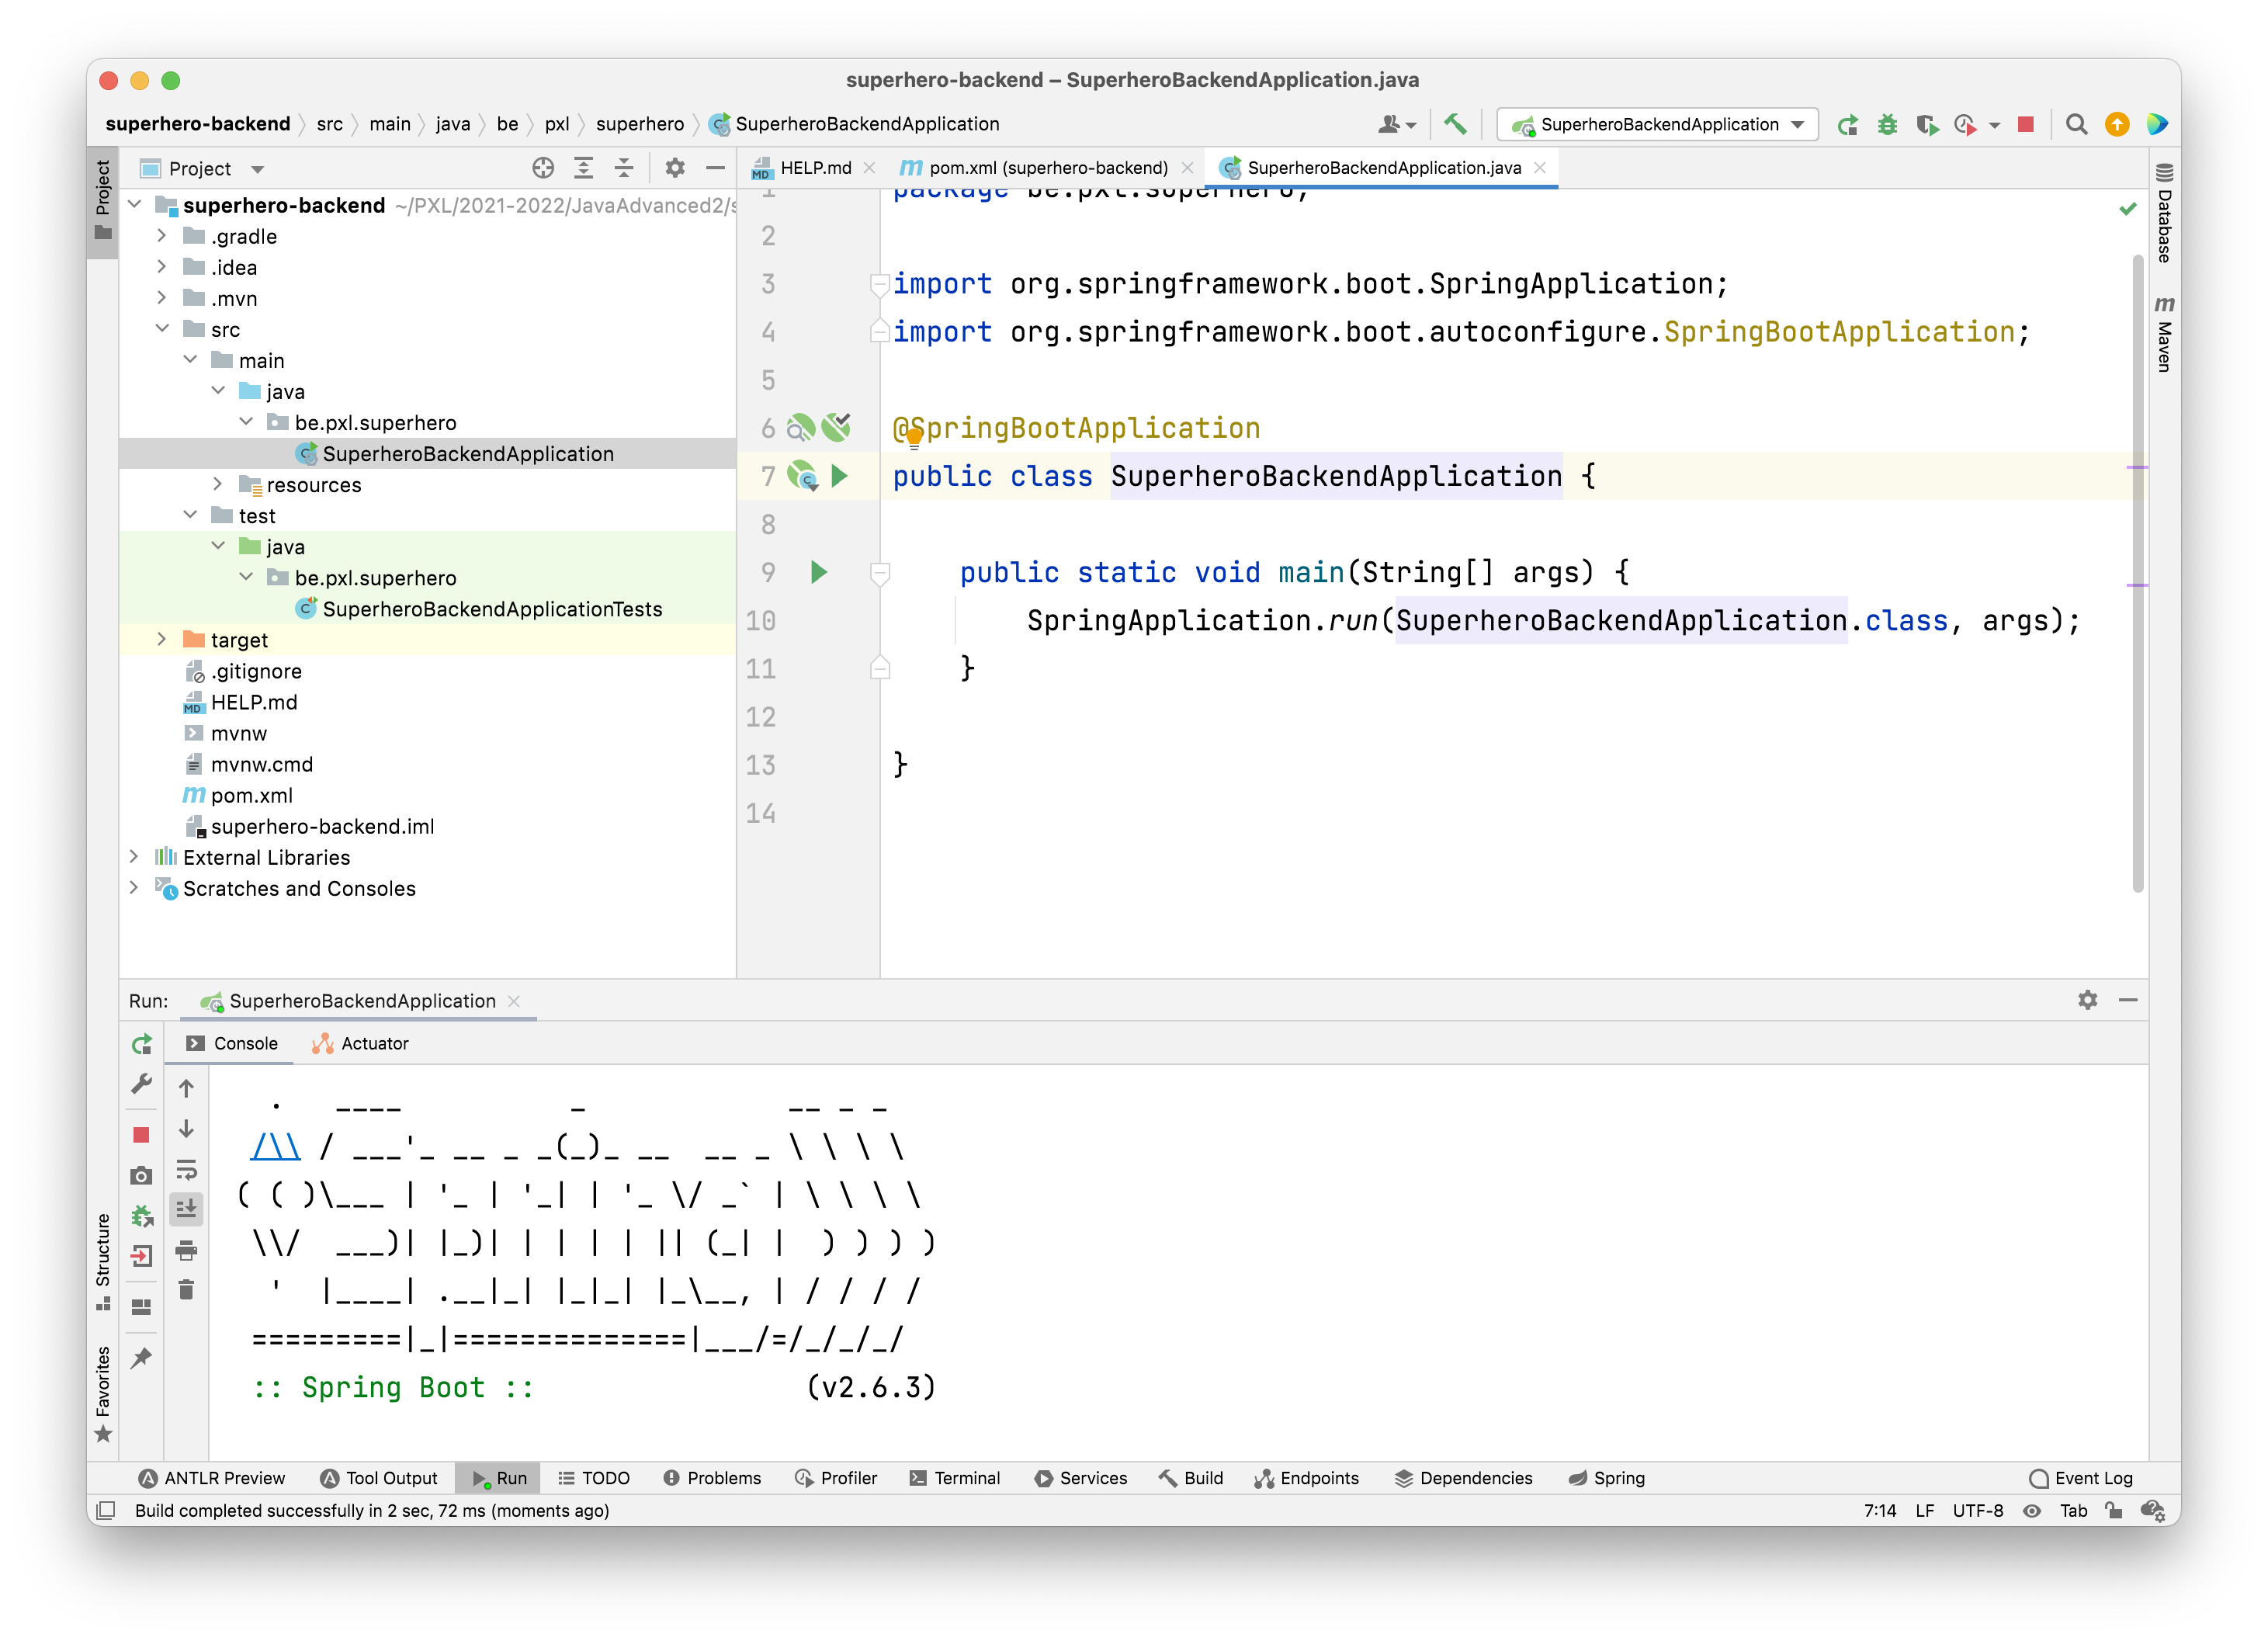
\includegraphics[width=\textwidth]{./images/chapter2/first-run.png}

Currently our Spring Boot application only shows a whitelabel error page. This error page is available when you perform a GET for URL \url{http://localhost:8080}.

\frame{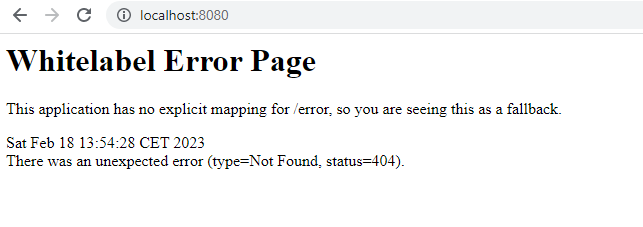
\includegraphics[width=\textwidth]{./images/chapter2/whitelabel_error_page.png}} 

Port 8080 is the default port. If this port is not available you will see an error message in Spring Boot's logging.

\begin{lstlisting}[frame=single]
***************************
APPLICATION FAILED TO START
***************************

Description:

Web server failed to start. Port 8080 was already in use.
\end{lstlisting}

The port number can be changed in the file application.properties. You have to add the property server.port here with the desired port number.

\begin{lstlisting}[frame=single]
server.port=8081
\end{lstlisting}

\section{De RestController}

Spring boot heeft een annotatie voorzien voor de Java Bean die verantwoordelijk is voor het afhandelen van HTTP requests nl @RestController. Spring boot heeft ook een annotatie @Controller, maar de @RestController zorgt ervoor dat het respons op het HTTP-request automatisch wordt omgezet (geserialiseerd) naar JSON of XML en wordt teruggestuurd naar de client.


\begin{lstlisting}[frame=single]
package be.pxl.demo.api;

import jakarta.annotation.PostConstruct;
import org.springframework.web.bind.annotation.GetMapping;
import org.springframework.web.bind.annotation.RestController;

import java.util.ArrayList;
import java.util.List;
import java.util.Random;

@RestController
@RequestMapping("/greetings")
public class GreetingController {

    private final List<String> messages = new ArrayList<>();
    private static final Random RANDOM = new Random();

    @PostConstruct
    public void init() {
        messages.add("Peek-a-boo!");
        messages.add("Howdy-doody!");
        messages.add("My name's Ralph, and I'm a bad guy.");
        messages.add("I come in peace!");
        messages.add("Put that cookie down!");

    }

    @GetMapping("/hello")
    public String doGreeting() {
        return messages.get(RANDOM.nextInt(messages.size()));
    }
}
\end{lstlisting}

De @RestController markeert de klasse GreetingController als een REST-controller.
De annotatie @RequestMapping("/greetings") specificeert het basispad voor alle requests die door deze controller worden afgehandeld.
@GetMapping("/hello") geeft aan dat de goGreeting-methode wordt uitgevoerd wanneer een HTTP GET-verzoek wordt gemaakt naar het pad "/greetings/hello". Het resultaat van deze methode wordt automatisch omgezet in tekst en teruggestuurd als de respons.

\begin{figure}[H]
  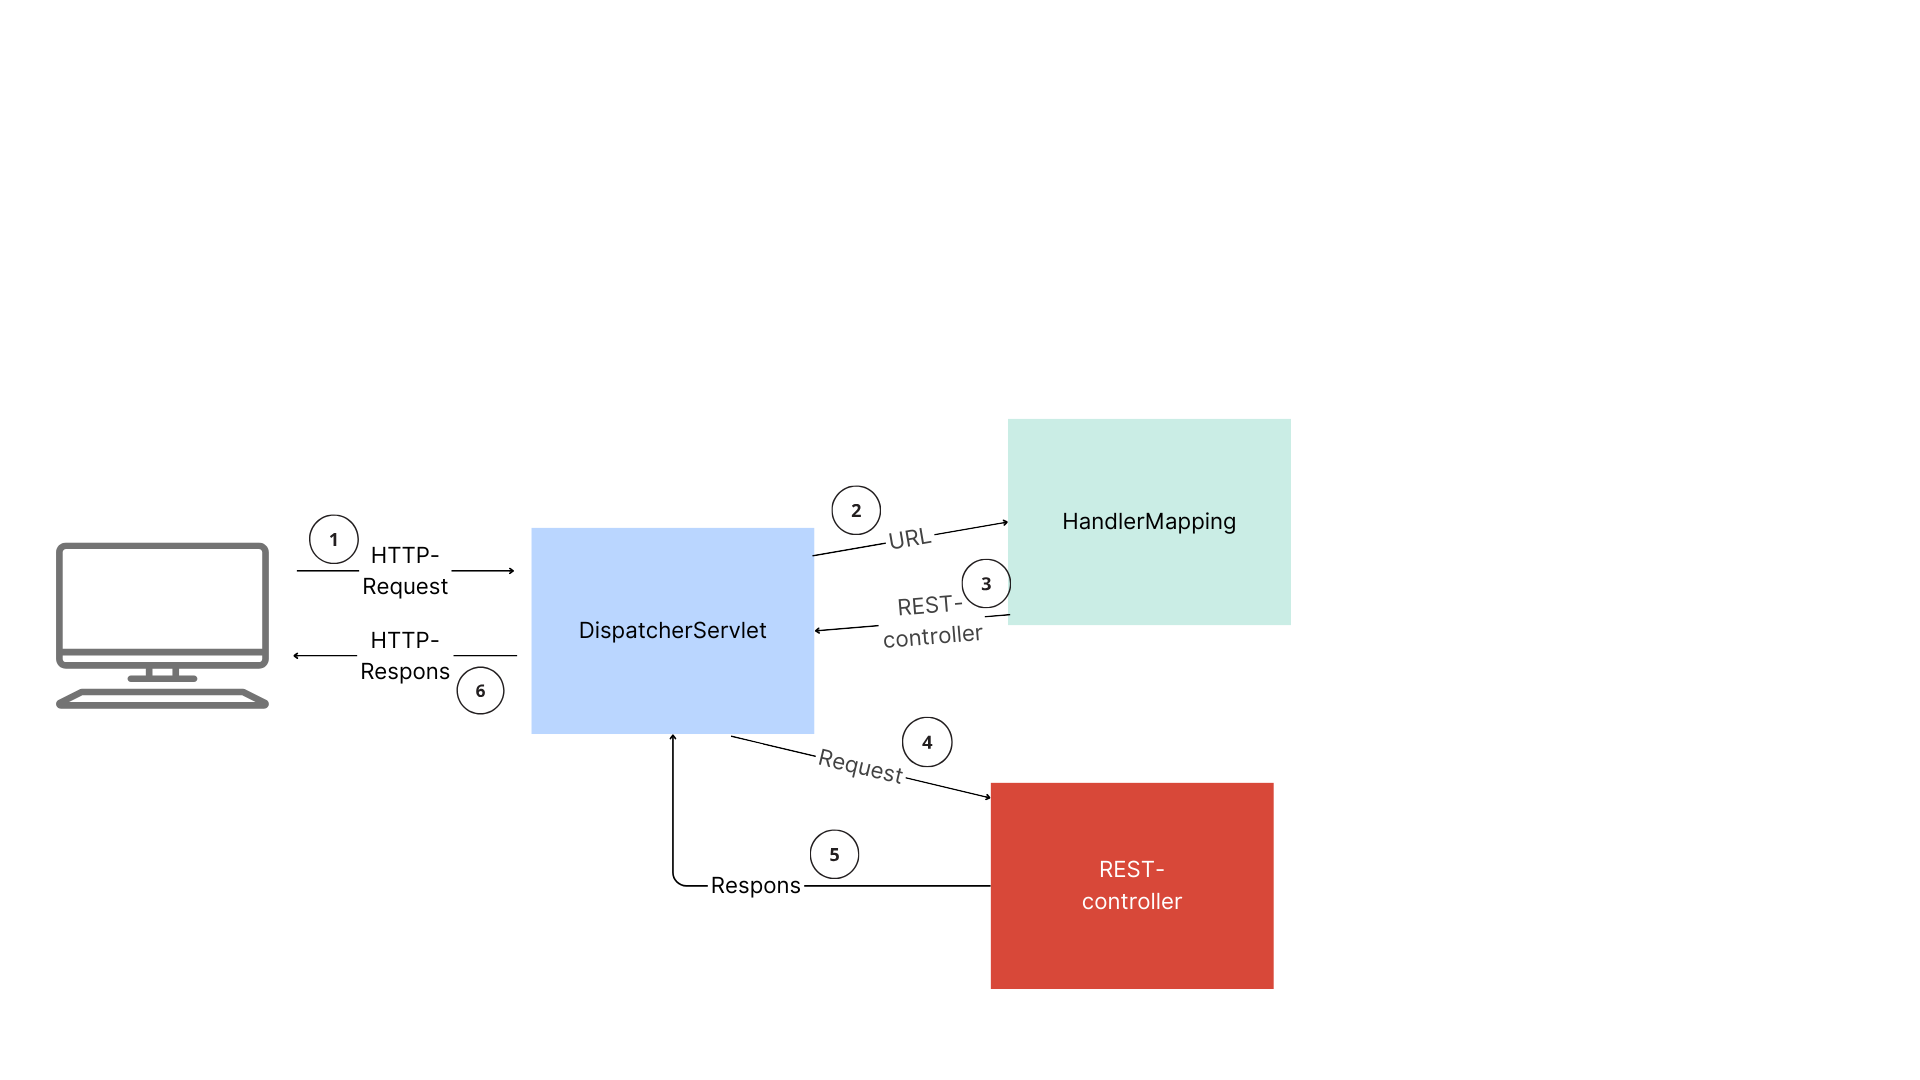
\includegraphics[width=\linewidth]{images/chapter-rest/dispatcherservlet.png}
  \caption{Een REST-verzoek afhandelen}
  \label{fig:test_passed}
\end{figure}

De component van Spring Boot die verantwoordelijk is dat een HTTP-request door de juiste REST-controller wordt afgehandeld is de DispatcherServlet.  De DispatcherServlet is onderdeel van Spring MVC.  De DispatcherServlet bepaalt welke controller een HTTP-request moet afhandelen,  hij geeft het request door aan de juiste controller en  verwerkt het respons van de controller om een HTTP-respons terug te sturen naar de client.

Om te achterhalen welke REST-controller verantwoordelijk is om een HTTP-request af te handelen raadpleegt de DispatcherServlet de HandlerMapping. De HandlerMapping is als het ware een kaart die URL's koppelt aan specifieke controllerklassen en methoden.
Op basis van de URL in het binnenkomende request bepaalt de DispatcherServlet welke controllerklasse en methode verantwoordelijk zijn voor het afhandelen van het request.


\begin{oefening}
Create the package \textit{be.pxl.demo.api}. Add the class \textbf{GreetingController} in this package. Restart the Spring Boot application and open the URL \url{http://localhost:8080/greetings/hello} in a browser. Voeg in de REST-controller een methode toe met de URI GET /greetings/daytime die de huidige dag en het tijdstip teruggeeft in het formaat 'Maandag 18 september 2023'.
\end{oefening}

\section{MusicPlaylist}

We gaan een nieuwe Spring Boot toepassing starten waarmee we een muziek playlist beheren. 

\begin{oefening}
Maak een nieuwe Spring boot toepassing MusicPlaylist. We gebruiken Spring MVC om een RESTful web applicatie te maken.  
\end{oefening}

\subsection{Een liedje toevoegen aan een playlist}

\begin{apiRoute}{post}{/playlist/songs}{Add a new song to the playlist.}
\begin{routeParameter}
	\noRouteParameter {no parameter }
\end{routeParameter}
\begin{routeRequest}{application/json}
\begin{routeRequestBody}
{
  "title": "Hello",
  "artist": "Adele",
  "duration_seconds": 293,
  "genre": "POP"
}
\end{routeRequestBody}
\end{routeRequest}
\begin{routeResponse}{application/json}
\begin{routeResponseItem}{200}{ok}
\end{routeResponseItem}
\end{routeResponse}
\end{apiRoute}


Om te beginnen hebben we de klasse Song nodig. 

\begin{lstlisting}[language=java,  frame=single]
public class Song {
    private String title;
    private String artist;
    @JsonProperty("duration_seconds")
    private int durationSeconds;
    private Genre genre;

    // Default constructor
    public Song() {
    }

    // Parameterized constructor
    public Song(String title, String artist, int durationSeconds, Genre genre) {
        this.title = title;
        this.artist = artist;
        this.durationSeconds = durationSeconds;
        this.genre = genre;
    }

    // Getter and setter methods
    public String getTitle() {
        return title;
    }

    public void setTitle(String title) {
        this.title = title;
    }

    public String getArtist() {
        return artist;
    }

    public void setArtist(String artist) {
        this.artist = artist;
    }

    public int getDurationSeconds() {
        return durationSeconds;
    }

    public void setDurationSeconds(int durationSeconds) {
        this.durationSeconds = durationSeconds;
    }

    public Genre getGenre() {
        return genre;
    }

    public void setGenre(Genre genre) {
        this.genre = genre;
    }

    @Override
    public String toString() {
        return "Song{" +
                "title='" + title + '\'' +
                ", artist='" + artist + '\'' +
                ", durationSeconds=" + durationSeconds +
                ", genre='" + genre + '\'' +
                '}';
    }
}
\end{lstlisting}


Nu gaan we de REST-controller implementeren.  We gaan hierin een methode voorzien die een POST op de URI /playlist/songs kan afhandelen.  Initieel gaan we enkel de titel in de loggegevens tonen. 

\begin{lstlisting}[language=java,  frame=single]
@RestController
@RequestMapping("/playlist/songs")
public class MusicPlaylistController {

	private static final Logger LOGGER = LoggerFactory.getLogger(MusicPlaylistController.class);

	@PostMapping
	public void addSong(@RequestBody Song song) {
		if (LOGGER.isInfoEnabled()) {
			LOGGER.info("Adding song [" + song.getTitle() + "]");
		}
	}
}
\end{lstlisting}

De liedjes die aan de playlist worden toegevoegd willen we bijhouden. Later zullen we ze wegschrijven in een databank, maar voorlopig gaan we ze bijhouden in een lijst.
Om dit mogelijk te maken gaan we een nieuwe Spring Bean toevoegen: de MusicPlaylistService.  

\begin{lstlisting}[language=java,  frame=single]
package be.pxl.demo;

import be.pxl.demo.domain.Song;
import org.springframework.stereotype.Service;

import java.util.ArrayList;
import java.util.List;

@Service
public class MusicPlaylistService {
	private final List<Song> myPlaylist = new ArrayList<>();

	public void addSong(Song song) {
		myPlaylist.add(song);
	}
}
\end{lstlisting}

De MusicPlaylistService wordt geannoteerd met @Service .
In onze Spring Boot applicaties gaan we steeds de business-logica implementeren in de service-laag.  De @Service annotatie wordt gebruikt voor de componenten (Spring Beans) in de service-laag.  Wanneer onze Spring Boot applicatie opstart wordt er exact \'e\'en instantie van de MusicPlaylistService aangemaakt in de ApplicationContext en deze instantie wordt tijdens de volledige levensduur van de toepassing gebruikt.  Dit noemen we de scope van de service en de default scope noemen we \textbf{singleton}. 
Dit betekent dat we \'e\'en enkele, gedeelde playlist hebben voor alle gebruikers.

Nu gaan we de MusicPlaylistService beschikbaar maken in de MusicPlaylistController.
We maken gebruik van \textbf{constructor injection}.  Zodra de instantie van de MusicPlaylistController door Spring Boot wordt aangemaakt, zal er eerst gezorgd worden dat de instantie MusicPlaylistService aangemaakt wordt. Deze instantie wordt dan achter de schermen meegegeven aan de constructor van de MusicPlaylistController. Zo kan ons MusicPlaylistController-object het MusicPlaylistService-object gebruiken.
Omdat er maar \'e\'en constructor is, is de annotatie @Autowired eigenlijk overbodig.

\begin{lstlisting}[language=java,  frame=single]
@RestController
@RequestMapping("/playlist/songs")
public class MusicPlaylistController {

	private static final Logger LOGGER = LoggerFactory.getLogger(MusicPlaylistController.class);
	private final MusicPlaylistService musicPlaylistService;

	@Autowired
	public MusicPlaylistController(MusicPlaylistService musicPlaylistService) {
		this.musicPlaylistService = musicPlaylistService;
	}

	@PostMapping
	public void addSong(@RequestBody Song song) {
		if (LOGGER.isInfoEnabled()) {
			LOGGER.info("Adding song [" + song.getTitle() + "]");
		}
		musicPlaylistService.addSong(song);
	}
}
\end{lstlisting}

Test nu het POST-verzoek.  Je kan Postman,  Insomnia of een andere tool gebruiken om een POST-verzoek naar de toepassing te sturen.  De toegevoegde liedjes gaan uiteraard verloren wanneer je de toepassing herstart. 

\begin{figure}[H]
  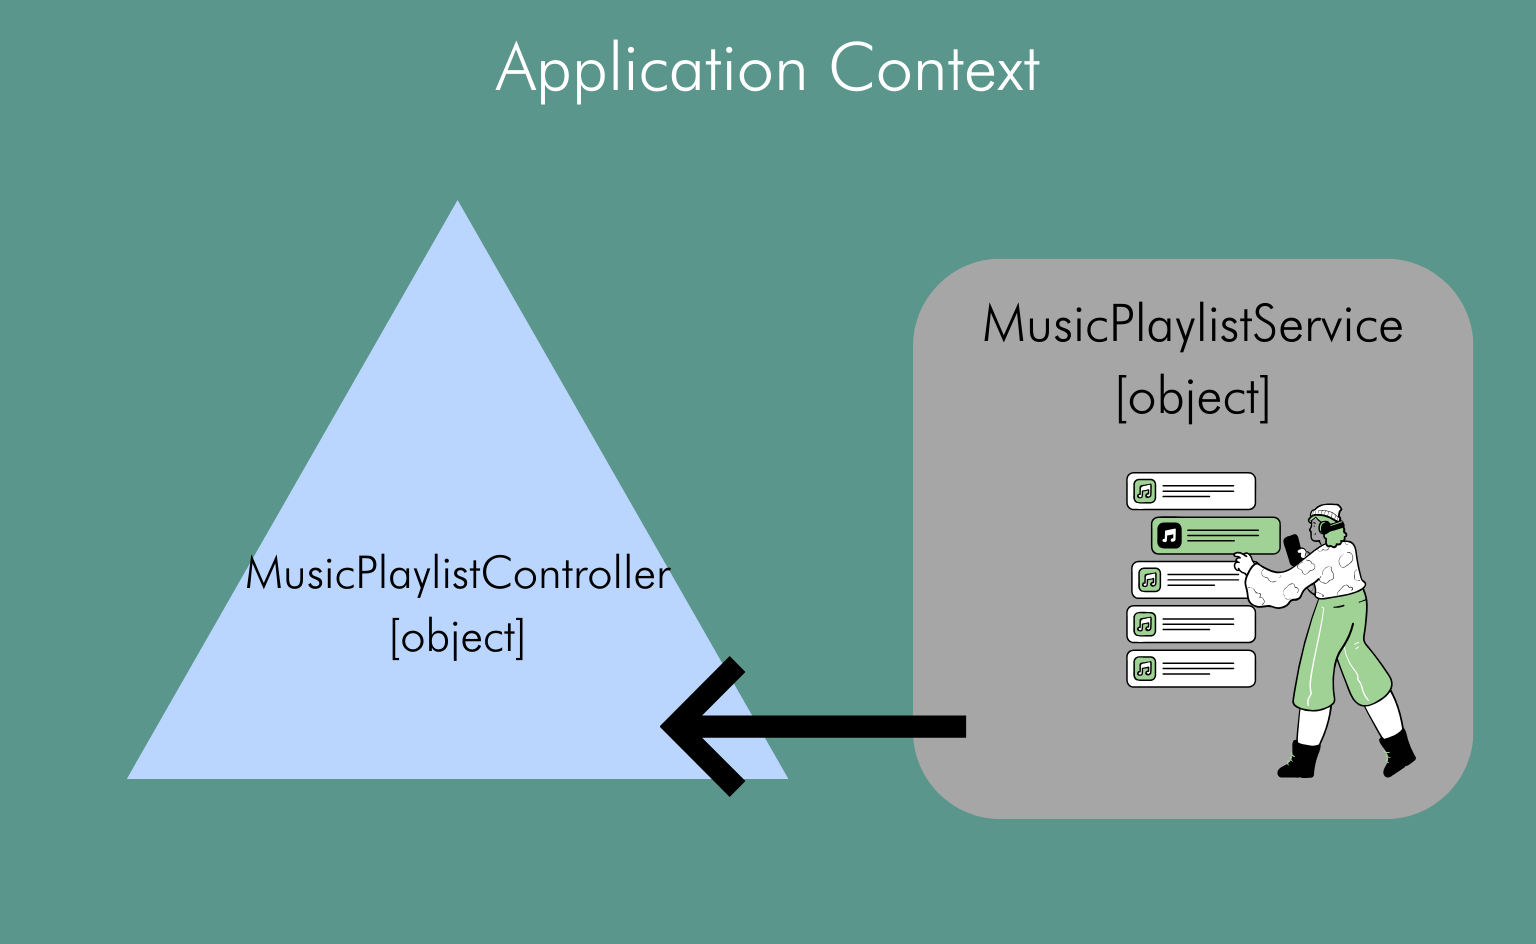
\includegraphics[width=\linewidth]{images/chapter-rest/applicationcontext_musicplaylist.png}
  \caption{Spring Beans in de Application Context}
  \label{fig:spring_beans_musicplaylist}
\end{figure}


\begin{figure}[H]
  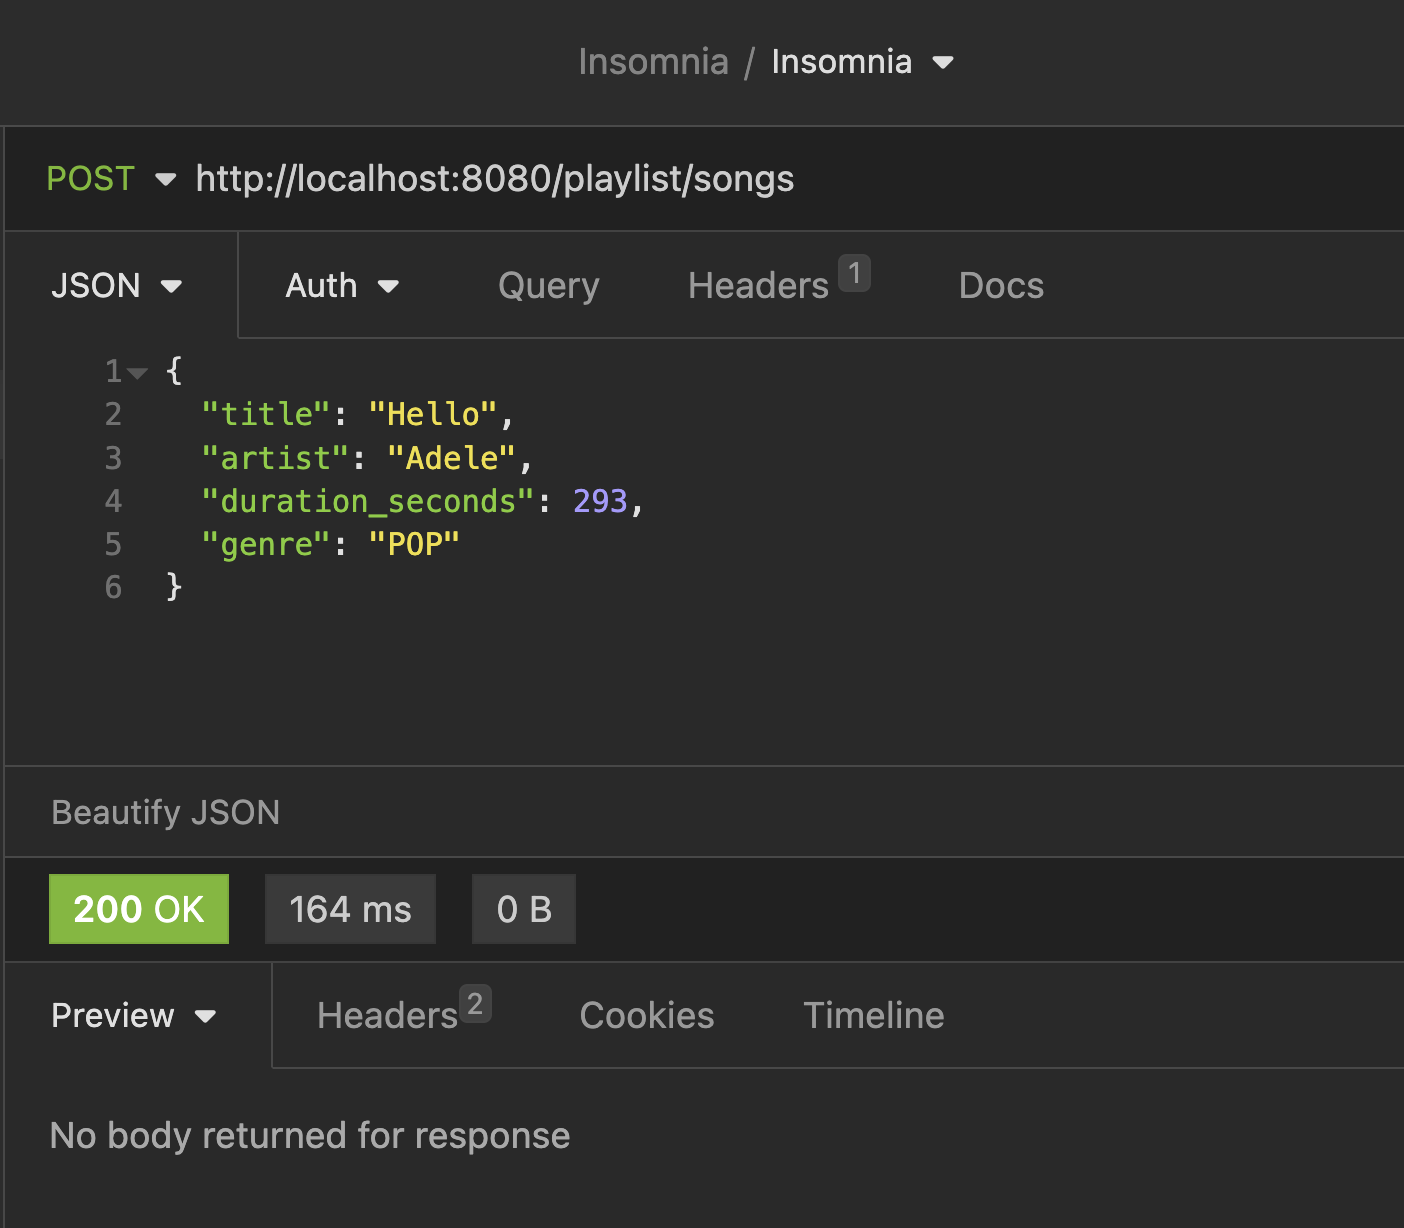
\includegraphics[width=\linewidth]{images/chapter-rest/insomnia_post.png}
  \caption{POST-verzoek met Insomnia}
  \label{fig:post_request}
\end{figure}

\subsection{De playlist opvragen}


\begin{apiRoute}{get}{/playlist/songs}{Retrieve all songs from the playlist}
\begin{routeParameter}
	\noRouteParameter {no parameter }
\end{routeParameter}
\begin{routeRequest}{application/json}
\end{routeRequest}
\begin{routeResponse}{application/json}
\begin{routeResponseItem}{200}{ok}
\begin{routeResponseItemBody}
[
	{
		"title": "Hello",
		"artist": "Adele",
		"genre": "POP",
		"duration_seconds": 293
	},
	{
		"title": "Shape of You",
		"artist": "Ed Sheeran",
		"genre": "POP",
		"duration_seconds": 233
	},
	{
		"title": "Umbrella",
		"artist": "Rihanna",
		"genre": "RNB",
		"duration_seconds": 264
	}
]
\end{routeResponseItemBody}
\end{routeResponseItem}
\end{routeResponse}
\end{apiRoute}


\begin{lstlisting}[language=java,  frame=single]
package be.pxl.demo;

import be.pxl.demo.domain.Song;
import org.springframework.stereotype.Service;

import java.util.ArrayList;
import java.util.List;

@Service
public class MusicPlaylistService {
	private final List<Song> myPlaylist = new ArrayList<>();

	public void addSong(Song song) {
		myPlaylist.add(song);
	}

	public List<Song> getSongs() {
		return myPlaylist;
	}
}
\end{lstlisting}


\begin{lstlisting}[language=java,  frame=single]
package be.pxl.demo.controller;

import be.pxl.demo.MusicPlaylistService;
import be.pxl.demo.domain.Song;
import org.slf4j.Logger;
import org.slf4j.LoggerFactory;
import org.springframework.beans.factory.annotation.Autowired;
import org.springframework.web.bind.annotation.GetMapping;
import org.springframework.web.bind.annotation.PostMapping;
import org.springframework.web.bind.annotation.RequestBody;
import org.springframework.web.bind.annotation.RequestMapping;
import org.springframework.web.bind.annotation.RestController;

import java.util.List;

@RestController
@RequestMapping("/playlist/songs")
public class MusicPlaylistController {

	private static final Logger LOGGER = LoggerFactory.getLogger(MusicPlaylistController.class);
	private final MusicPlaylistService musicPlaylistService;

	@Autowired
	public MusicPlaylistController(MusicPlaylistService musicPlaylistService) {
		this.musicPlaylistService = musicPlaylistService;
	}

	@PostMapping
	public void addSong(@RequestBody Song song) {
		if (LOGGER.isInfoEnabled()) {
			LOGGER.info("Adding song [" + song.getTitle() + "]");
		}
		musicPlaylistService.addSong(song);
	}

	@GetMapping
	public List<Song> getSongs() {
		return musicPlaylistService.getSongs();
	}
}
\end{lstlisting}

\subsection{Liedjes van \'e\'en genre}


 
 \begin{apiRoute}{get}{/playlist/songs/\{genre\}}{Retrieve all songs from the playlist with the given genre}
\begin{routeParameter}
	\routeParamItem{genre}{the requested genre}
\end{routeParameter}
\begin{routeRequest}{application/json}
\end{routeRequest}
\begin{routeResponse}{application/json}
\begin{routeResponseItem}{200}{ok}
\begin{routeResponseItemBody}
[
	{
		"title": "Hello",
		"artist": "Adele",
		"genre": "POP",
		"duration_seconds": 293
	},
	{
		"title": "Shape of You",
		"artist": "Ed Sheeran",
		"genre": "POP",
		"duration_seconds": 233
	}
]
\end{routeResponseItemBody}
\end{routeResponseItem}
\end{routeResponse}
\end{apiRoute}


\begin{lstlisting}[language=java,  frame=single]
package be.pxl.demo.controller;

import be.pxl.demo.MusicPlaylistService;
import be.pxl.demo.domain.Genre;
import be.pxl.demo.domain.Song;
import org.slf4j.Logger;
import org.slf4j.LoggerFactory;
import org.springframework.beans.factory.annotation.Autowired;
import org.springframework.web.bind.annotation.GetMapping;
import org.springframework.web.bind.annotation.PathVariable;
import org.springframework.web.bind.annotation.PostMapping;
import org.springframework.web.bind.annotation.RequestBody;
import org.springframework.web.bind.annotation.RequestMapping;
import org.springframework.web.bind.annotation.RestController;

import java.util.List;

@RestController
@RequestMapping("/playlist/songs")
public class MusicPlaylistController {

	private static final Logger LOGGER = LoggerFactory.getLogger(MusicPlaylistController.class);
	private final MusicPlaylistService musicPlaylistService;

	@Autowired
	public MusicPlaylistController(MusicPlaylistService musicPlaylistService) {
		this.musicPlaylistService = musicPlaylistService;
	}

	@PostMapping
	public void addSong(@RequestBody Song song) {
		if (LOGGER.isInfoEnabled()) {
			LOGGER.info("Adding song [" + song.getTitle() + "]");
		}
		musicPlaylistService.addSong(song);
	}

	@GetMapping
	public List<Song> getSongs() {
		return musicPlaylistService.getSongs();
	}

	@GetMapping("{genre}")
	public List<Song> getSongs(@PathVariable Genre genre) {
		return musicPlaylistService.getSongsByGenre(genre);
	}
}
\end{lstlisting}

\begin{lstlisting}[language=java,  frame=single]
package be.pxl.demo;

import be.pxl.demo.domain.Genre;
import be.pxl.demo.domain.Song;
import org.springframework.stereotype.Service;

import java.util.ArrayList;
import java.util.List;

@Service
public class MusicPlaylistService {
	private final List<Song> myPlaylist = new ArrayList<>();

	public void addSong(Song song) {
		myPlaylist.add(song);
	}

	public List<Song> getSongs() {
		return myPlaylist;
	}

	public List<Song> getSongsByGenre(Genre genre) {
		List<Song> response = new ArrayList<>();
		for (Song song : myPlaylist) {
			if (song.getGenre() == genre) {
				response.add(song);
			}
		}
		return response;
	}
}
\end{lstlisting}


\subsection{Gegevens van een liedje aanpassen}

Als je een nieuwe song in de playlist toevoegt, dan word deze steeds achteraan in de lijst toegevoegd. We kunnen nu de gegevens van een liedje op een bepaalde positie in de lijst gaan overschrijven of aanpassen.

We gaan hiervoor een PUT-verzoek gebruiken.

\begin{lstlisting}
package be.pxl.demo.controller;

import be.pxl.demo.MusicPlaylistService;
import be.pxl.demo.domain.Genre;
import be.pxl.demo.domain.Song;
import org.slf4j.Logger;
import org.slf4j.LoggerFactory;
import org.springframework.beans.factory.annotation.Autowired;
import org.springframework.web.bind.annotation.DeleteMapping;
import org.springframework.web.bind.annotation.GetMapping;
import org.springframework.web.bind.annotation.PathVariable;
import org.springframework.web.bind.annotation.PostMapping;
import org.springframework.web.bind.annotation.PutMapping;
import org.springframework.web.bind.annotation.RequestBody;
import org.springframework.web.bind.annotation.RequestMapping;
import org.springframework.web.bind.annotation.RestController;

import java.util.List;

@RestController
@RequestMapping("/playlist/songs")
public class MusicPlaylistController {

	private static final Logger LOGGER = LoggerFactory.getLogger(MusicPlaylistController.class);
	private final MusicPlaylistService musicPlaylistService;

	@Autowired
	public MusicPlaylistController(MusicPlaylistService musicPlaylistService) {
		this.musicPlaylistService = musicPlaylistService;
	}

	@PostMapping
	public void addSong(@RequestBody Song song) {
		if (LOGGER.isInfoEnabled()) {
			LOGGER.info("Adding song [" + song.getTitle() + "]");
		}
		musicPlaylistService.addSong(song);
	}

	@GetMapping
	public List<Song> getSongs() {
		return musicPlaylistService.getSongs();
	}

	@GetMapping("/{genre}")
	public List<Song> getSongs(@PathVariable Genre genre) {
		return musicPlaylistService.getSongsByGenre(genre);
	}

	@PutMapping("/{index}")
	public void updateSong(@PathVariable int index, @RequestBody Song song) {
		musicPlaylistService.updateSong(index, song);
	}

	@DeleteMapping("/{index}")
	public void updateSong(@PathVariable int index) {
		musicPlaylistService.deleteSong(index);
	}
}
\end{lstlisting}

\begin{lstlisting}
package be.pxl.demo;

import be.pxl.demo.domain.Genre;
import be.pxl.demo.domain.Song;
import org.springframework.stereotype.Service;

import java.util.ArrayList;
import java.util.List;

@Service
public class MusicPlaylistService {
	private final List<Song> myPlaylist = new ArrayList<>();

	public void addSong(Song song) {
		myPlaylist.add(song);
	}

	public List<Song> getSongs() {
		return myPlaylist;
	}

	public List<Song> getSongsByGenre(Genre genre) {
		List<Song> response = new ArrayList<>();
		for (Song song : myPlaylist) {
			if (song.getGenre() == genre) {
				response.add(song);
			}
		}
		return response;
	}

	public void updateSong(int index, Song song) {
		myPlaylist.set(index, song);
	}

	public void deleteSong(int index) {
		myPlaylist.remove(index);
	}
}
\end{lstlisting}

\subsection{Een liedje verwijderen}

Om een liedje op een opgegeven positie uit de playlist te verwijderen gaan we een DELETE-verzoek implementeren.


\begin{lstlisting}
package be.pxl.demo.controller;

import be.pxl.demo.MusicPlaylistService;
import be.pxl.demo.domain.Genre;
import be.pxl.demo.domain.Song;
import org.slf4j.Logger;
import org.slf4j.LoggerFactory;
import org.springframework.beans.factory.annotation.Autowired;
import org.springframework.web.bind.annotation.DeleteMapping;
import org.springframework.web.bind.annotation.GetMapping;
import org.springframework.web.bind.annotation.PathVariable;
import org.springframework.web.bind.annotation.PostMapping;
import org.springframework.web.bind.annotation.PutMapping;
import org.springframework.web.bind.annotation.RequestBody;
import org.springframework.web.bind.annotation.RequestMapping;
import org.springframework.web.bind.annotation.RestController;

import java.util.List;

@RestController
@RequestMapping("/playlist/songs")
public class MusicPlaylistController {

	private static final Logger LOGGER = LoggerFactory.getLogger(MusicPlaylistController.class);
	private final MusicPlaylistService musicPlaylistService;

	@Autowired
	public MusicPlaylistController(MusicPlaylistService musicPlaylistService) {
		this.musicPlaylistService = musicPlaylistService;
	}

	@PostMapping
	public void addSong(@RequestBody Song song) {
		if (LOGGER.isInfoEnabled()) {
			LOGGER.info("Adding song [" + song.getTitle() + "]");
		}
		musicPlaylistService.addSong(song);
	}

	@GetMapping
	public List<Song> getSongs() {
		return musicPlaylistService.getSongs();
	}

	@GetMapping("/{genre}")
	public List<Song> getSongs(@PathVariable Genre genre) {
		return musicPlaylistService.getSongsByGenre(genre);
	}

	@PutMapping("/{index}")
	public void updateSong(@PathVariable int index, @RequestBody Song song) {
		musicPlaylistService.updateSong(index, song);
	}

	@DeleteMapping("/{index}")
	public void updateSong(@PathVariable int index) {
		musicPlaylistService.deleteSong(index);
	}
}
\end{lstlisting}


\begin{lstlisting}
package be.pxl.demo;

import be.pxl.demo.domain.Genre;
import be.pxl.demo.domain.Song;
import org.springframework.stereotype.Service;

import java.util.ArrayList;
import java.util.List;

@Service
public class MusicPlaylistService {
	private final List<Song> myPlaylist = new ArrayList<>();

	public void addSong(Song song) {
		myPlaylist.add(song);
	}

	public List<Song> getSongs() {
		return myPlaylist;
	}

	public List<Song> getSongsByGenre(Genre genre) {
		List<Song> response = new ArrayList<>();
		for (Song song : myPlaylist) {
			if (song.getGenre() == genre) {
				response.add(song);
			}
		}
		return response;
	}

	public void updateSong(int index, Song song) {
		myPlaylist.set(index, song);
	}

	public void deleteSong(int index) {
		myPlaylist.remove(index);
	}
}
\end{lstlisting}


\section{Gegevens valideren}



\begin{oefening}\textbf{Huizenjacht}
We maken een Spring Boot toepassing om het aanbod op de huizenmarkt te tonen.
Ontwikkel een RESTful web toepassing met de volgende endpoints.

Een huis wordt voorgesteld als een resource met volgende eigenschappen:

\begin{itemize}
  \item \texttt{code} (string): Unieke identificatie van het huis.
  \item \texttt{name} (string): De naam of beschrijving van het huis.
  \item \texttt{status} (enum): FOR\_SALE en SOLD.
  \item \texttt{city} (string): Stad van het huis.
  \item \texttt{price} (double): De vraagprijs van het huis.
\end{itemize}

\section{REST Endpoints}

\begin{apiRoute}{post}{/houses}{Create a new house.}
\begin{routeParameter}
	\noRouteParameter {no parameter }
\end{routeParameter}
\begin{routeRequest}{application/json}
\begin{routeRequestBody}
{
  "code": "HAS_001",
  "name": "Beautiful house in the city",
  "city": "Hasselt",
  "price": 250000
}
\end{routeRequestBody}
\end{routeRequest}
\begin{routeResponse}{application/json}
\begin{routeResponseItem}{200}{ok}
\end{routeResponseItem}
\end{routeResponse}
\end{apiRoute}


\begin{apiRoute}{post}{/houses/\{code\}}{Update the status of the house with the given code.}
\begin{routeParameter}
	\noRouteParameter {no parameter }
\end{routeParameter}
\begin{routeRequest}{application/json}
\begin{routeRequestBody}
{
  "code": "HAS_001",
  "name": "Beautiful house in the city",
  "city": "Hasselt",
  "price": 250000
}
\end{routeRequestBody}
\end{routeRequest}
\begin{routeResponse}{application/json}
\begin{routeResponseItem}{200}{ok}
\end{routeResponseItem}
\end{routeResponse}
\end{apiRoute}

\begin{api}
  \method{PUT}{/houses/\{id\}}{Update House}
  \request{JSON}{A JSON object with the \texttt{status} attribute to update the house's status.}
  \response{JSON}{The updated house object.}
\end{api}

\begin{api}
  \method{GET}{/houses}{Get All Houses}
  \response{JSON}{A list of all available houses with attributes \texttt{id}, \texttt{name}, \texttt{status}, and \texttt{price}.}
\end{api}

\begin{api}
  \method{DELETE}{/houses/\{id\}}{Delete House}
  \response{JSON}{A confirmation that the house has been deleted.}
\end{api}

\section{Examples of JSON Data}

Here are some examples of JSON data that can be used for the API operations:

\subsection{Create New House (POST)}

\begin{verbatim}
{
  "name": "Beautiful house in the city",
  "status": "for sale",
  "price": 250000
}
\end{verbatim}

\subsection{Update House (PUT)}

\begin{verbatim}
{
  "status": "sold"
}
\end{verbatim}

\subsection{Response after GET Request (GET)}

\begin{verbatim}
[
  {
    "id": 1,
    "name": "Beautiful house in the city",
    "status": "sold",
    "price": 250000
  },
  {
    "id": 2,
    "name": "Cozy bungalow",
    "status": "for sale",
    "price": 180000
  }
]
\end{verbatim}

\end{oefening}